\documentclass[12pt,aspectratio=169]{beamer}
\usepackage{subcaption}
\usefonttheme{serif}
\setbeamertemplate{navigation symbols}{}\date{}
\begin{document}\begin{frame}[plain,t]
Alpha before.
\begin{figure}
\begin{subfigure}[b]{.42\textwidth}\centering
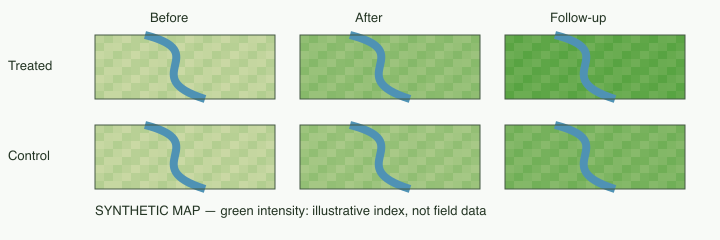
\includegraphics[width=\linewidth]{../breadth-decks/assets/river-transects.png}
\caption{A wrapped panel caption explains how the full river map was sampled.}
\end{subfigure}\hfill
\begin{subfigure}[b]{.52\textwidth}\centering
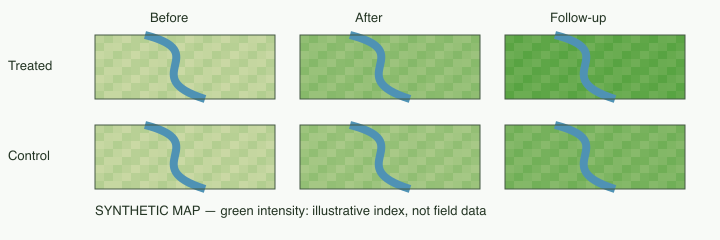
\includegraphics[width=\linewidth]{../breadth-decks/assets/river-transects.png}
\caption{Second.}
\end{subfigure}
\caption{Omega caption.}
\end{figure}
After the figure.
\end{frame}\end{document}
